\documentclass{article}
\usepackage{hyperref}
\usepackage{enumitem}
\usepackage{graphicx}
\usepackage{amsmath}
\usepackage{mathpazo}

\begin{document}
\title{ECE574 Final Project Report: \\ Reconfigurable Partially Pipelined RAM-based FIR Filter}
\author{Brian B Cheng \\ Rutgers University Department of Electrical and Computer Engineering}


\date{}
\maketitle


\section{Abstract}
    This report presents a Verilog implementation of a reconfigurable Finite Impulse Response (FIR) filter designed for heterogeneous FPGAs.
    The model is highly flexible, with customizable data width, filter depth, and the number of parallel multiply-accumulate (MAC) pipelines, all configurable through top-level parameters.
    The filter modifies the traditional direct-form FIR structure by replacing the input shift register with RAM elements and the stationary weights with ROM elements. 
    Input samples are written to RAM as new samples arrive, with the write address counting downward.
    Concurrently, weights and samples are read from the ROMs and RAMs into their respective MAC units, with read addresses counting upward. 
    This counter-directional address counting achieves the "shift register" effect of a traditional direct-form filter.
    The method is demonstrated with a 256-tap FIR filter featuring a 24-bit data width and eight parallel MAC pipelines. 
    A testbench simulation provides a noisy sine wave as input, demonstrating the filter's performance in producing a clean sine wave output, verified in the waveform diagrams.

\section{Introduction}
    Finite Impulse Response (FIR) filters are commonly used in digital signal processing to remove unwanted frequencies from a noisy signal while preserving the desired frequency bands.
    They are particularly well-suited for implementation on FPGAs due to their unique balance between low latency, parallelism, and hardware flexibility.
    When implementing FIR filters on FPGAs, several key design constraints must be considered.
    Hardware constraints include the number utilization of multipliers (which are costly), adders, and registers used.
    Performance constraints include throughput, output latency, and placement area.
    Efficient design requires careful trade-offs between these constraints to meet the application's performance and resource requirements.
    This report presents an FIR filter that prioritizes placement area by opting for RAM and ROM elements instead of registers, and sacrifices low-latency for higher throughput via extensive usage of parallel pipelining.
    At the same time however, the usage of RAM and ROM instead of registers hinders the higher throughput as memory access throughput is slower than register throughput.
    Thus, the main benefit of this implementation is the placement profile on the FPGA chip.
    A smaller placement profiles can yield fewer wire nets and less congested routing, which may also contribute to lower power usage.

\section{Data Description}
    As mentioned in the Introduction, the purpose of a FIR Filter is to filter out unwanted frequency bands from an input signal and provide an output signal containing only the desired frequency bands.
    This project presents a low pass filter with a cutoff frequency of 2KHz.
    Thus, to verify the filter, we supply a synthetic noisy signal containing frequencies below and above 2KHz and observe the output signal to see if the filter correctly filters out frequencies above 2KHz.
    To create this synthetic signal, we use Python to generate a Verilog header file containing the sine signal samples in hexadecimal format.
    We use the \texttt{`include "filename.vh"} compiler directive in our testbench SystemVerilog code to import the Python-generated input samples.
    All data signals in this implementation are 24-bit signed with fixed point representation Q1.23, meaning 1 sign bit, zero whole bits, and 23 fractional bits.
    Thus, the range of all data signals, including the weights, is between negative one and positive one.
    Shown in Equation~\ref{eq:sine} and Figure~\ref{fig:sine} is the formula and graph of the noisy sine wave, with the desired 200Hz sine wave added with an unwanted 5KHz sine wave noise.
    The sampling frequency is 44\,\text{kHz}, meaning the sampling period is \( 22.273 \times 10^{-6} \) seconds.

    \begin{equation}
        \text{input\_signal}(t) = 0.2 \cdot \sin(2 \pi f_{\text{low}} t)
        + 0.1 \cdot \sin(2 \pi f_{\text{high}} t)
        \label{eq:sine}
    \end{equation}
    \[
    \begin{aligned}
        f_{\text{low}} &= 200 \, \text{Hz}, & f_{\text{high}} &= 5 \, \text{KHz} \\
    \end{aligned}
    \]
    \begin{figure}
        \centering
        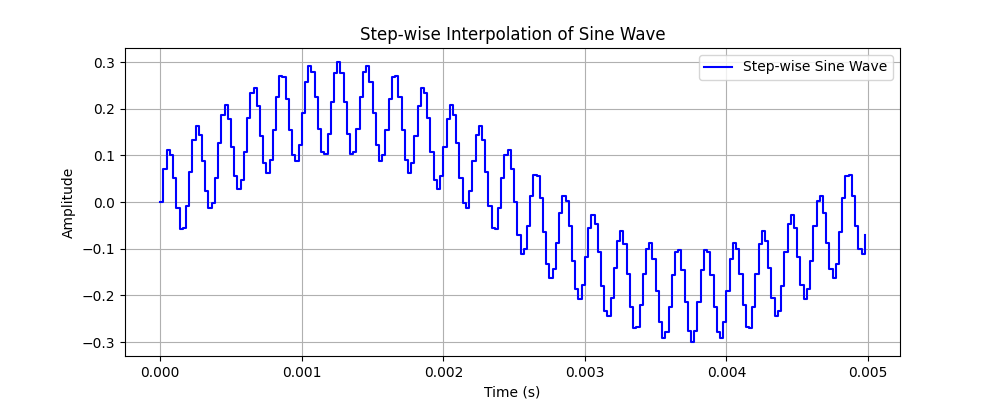
\includegraphics[width=1.00\textwidth]{figures/sine.png}
        \caption{Noisy input signal over 220 samples}\label{fig:sine}
    \end{figure}

    In similar fashion, we generate the 256 filter weights in Python using scipy's \texttt{firwin()} function.
    We store the weights in hexadecimal format in \texttt{.mem} files, one \texttt{.mem} file for each MAC pipeline.
    Each MAC operates on their unique subvector of the whole weight vector.
    We use Xilinx's XPM macro to instantiate ROM elements and initialize the memories with their respective \texttt{.mem} files.
    It is generally good practice to use vendor-specific macros instead of hand written memories to ensure correct memory behavior.
    Shown in Figure~\ref{fig:weights} below is the function call and plot of filter weights.

    \begin{verbatim}
        filter_depth = 256
        cutoff_freq = 2000
        sample_rate = 44000
        normalized_cutoff = cutoff_freq / (sample_rate / 2)
        firwin(filter_depth, normalized_cutoff)
    \end{verbatim}
    \begin{figure}
        \centering
        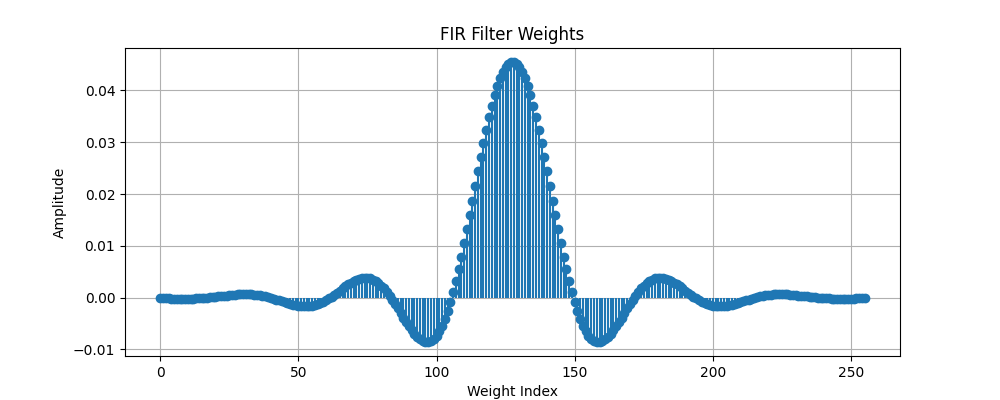
\includegraphics[width=1.00\textwidth]{figures/fir_coeff.png}
        \caption{256 filter weights for 44KHz sampling frequency and 2KHz cutoff frequency}\label{fig:weights}
    \end{figure}

\section{Method Description}
    \begin{figure}
        \centering
        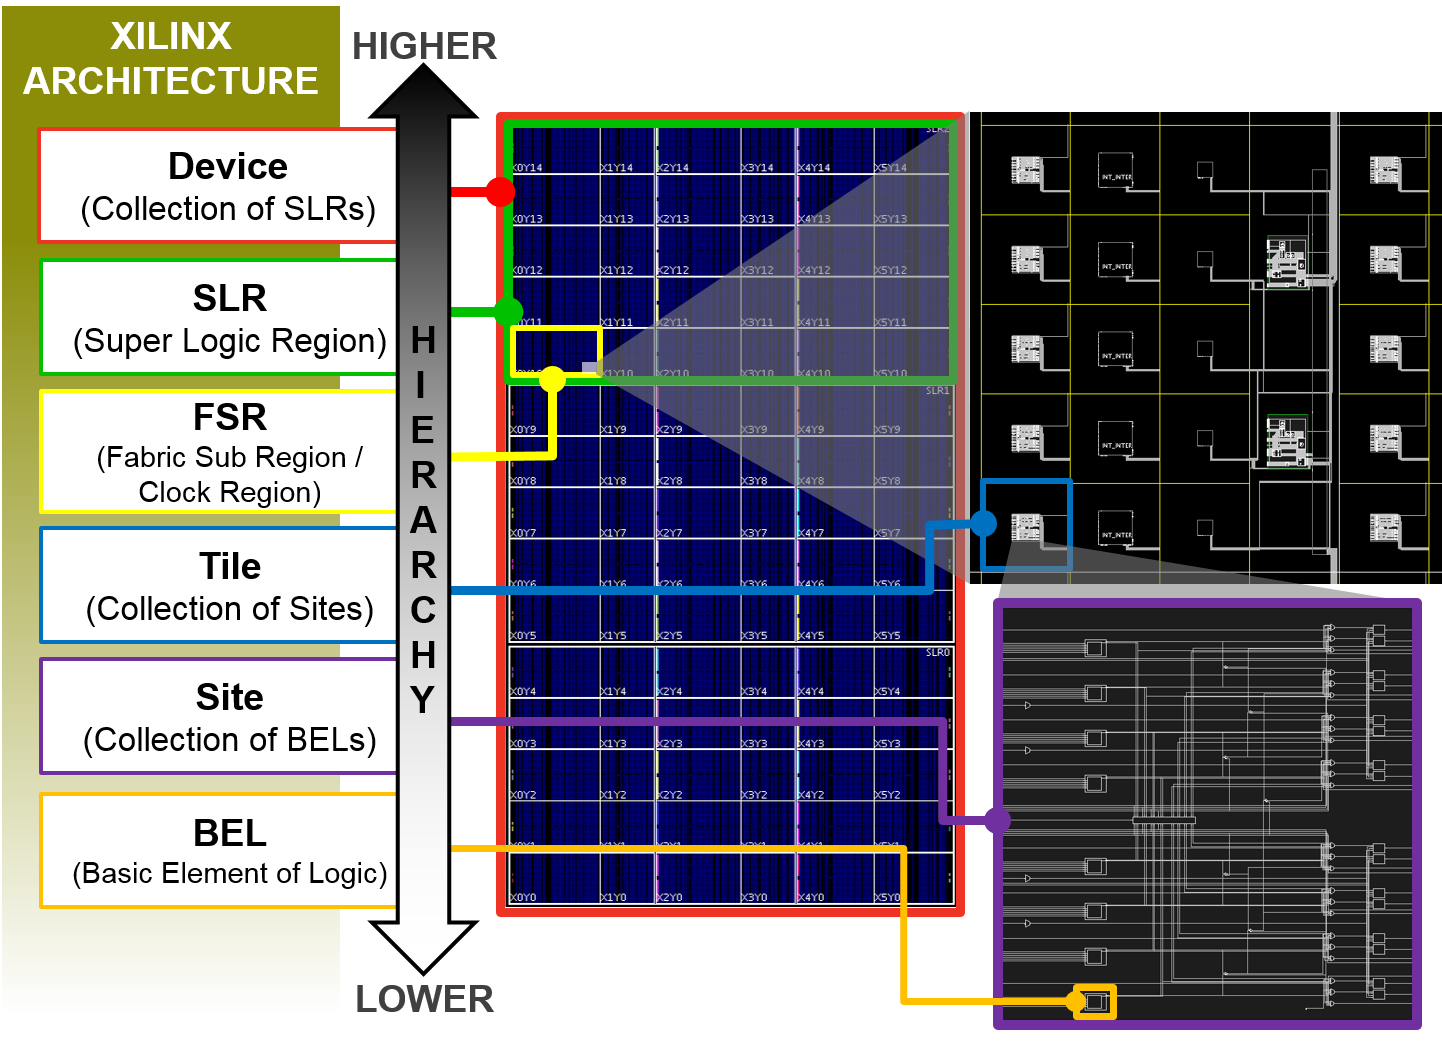
\includegraphics[width=1.00\textwidth]{figures/hierarchy.png}
        \caption{Xilinx FPGA Architecture Hierarchy}\label{fig:hierarchy}
    \end{figure}
    \subsection{Why Choose a RAM-Based Shift Register Over a Flip-Flop-Based Shift Register?}
    A critical decision in this design is replacing a traditional flip-flop-based shift register with a RAM-based implementation.
    This choice is motivated mainly by reducing CLB usage in favor of BRAM and reducing the area profile of the shift register.
    This, I theorize, improves the placement profile on the FPGA chip, and reduces the total number of wire nets which can alleviate routing congestion in the programmable interconnects.
    These two benefits overall contributes to a better Quality of Result (QoR) given that the performance specifications are met.
    The usage of BRAMs over registers can also theoretically reduce power usage as vendor-specific memory macros are highly optimized in modern FPGAs.

    For a 24-bit signal, each filter tap requires 24 registers.
    For instance, implementing a 256-tap FIR filter with 24-bit signals demands:
    \[
        256 \, \text{taps} \times 24 \, \text{bits/tap} = 6144 \, \text{flip-flops}.
    \]
    In a typical low-end Xilinx FPGA, such as the xc7z020, the available resources include \textbf{6650 configurable logic block (CLB) tiles}.
    Each CLB contains two logic sites, which can either be both SLICELs or a combination of one SLICEL and one SLICEM.
    The key difference between SLICEL and SLICEM is that SLICEM can reconfigure its lookup tables (LUTs) to function as small local RAMs, known as ``distributed RAM.''
    The xc7z020 provides a total of \textbf{8950 SLICELs} and \textbf{4350 SLICEMs}, summing to \textbf{13,300 logic sites} across all CLBs.
    Each logic site, regardless of type, contains \textbf{8 flip-flops}, meaning each CLB tile has \textbf{16 flip-flops}.
    To implement the shift register using flip-flops:
    \[
        \frac{6144 \, \text{flip-flops}}{16 \, \text{flip-flops/CLB}} = 384 \, \text{CLBs}.
    \]
    On the other hand, block RAM (BRAM) tiles provide a more resource-efficient alternative.
    Each BRAM tile contains \textbf{3 memory sites} (2 $\times$ 18Kb banks and 1 $\times$ 36Kb bank) that can be configured as RAM, ROM, or FIFO.
    A single BRAM tile occupies approximately the same space as \textbf{10 CLBs}.
    For an 8-pipeline FIR filter, the design requires \textbf{8 RAMs} (for input samples) and \textbf{8 ROMs} (for weights), totaling \textbf{16 memory elements}.
    With \textbf{3 memory sites per BRAM tile}, this requires:
    \[
        \frac{16 \, \text{memory elements}}{3 \, \text{memory sites per BRAM}} = 6 \, \text{BRAM tiles}.
    \]
    In terms of CLB-equivalent space, these 6 BRAM tiles occupy:
    \[
        6 \, \text{BRAM tiles} \times 10 \, \text{CLBs/BRAM} = 60 \, \text{CLBs}.
    \]
    By opting for a RAM-based shift register, the design trades the \textbf{384 CLBs} required for a flip-flop-based implementation for just \textbf{60 CLBs}, resulting in a significant reduction in logic site utilization.
    This trade-off demonstrates the value of leveraging the specialized memory resources available on FPGAs, such as BRAM, to implement resource-intensive designs efficiently.
    With a smaller floorplanning profile (also known as a PBlock size), we can dedicate the freed up logic sites to other parts of the system design.
    This also allows us to pack more FIR filters in parallel should the system design operate on multiple signal channels.
    Refer to Figure~\ref{fig:CLB_BRAM} to see a space profile comparison between BRAMs and CLBs.
    All of this of course comes with the tradeoffs mentioned earlier, and obviously, if the system is memory intensive elsewhere in the design, the RAM-based FIR filter might not be feasible.
    \begin{figure}
        \centering
        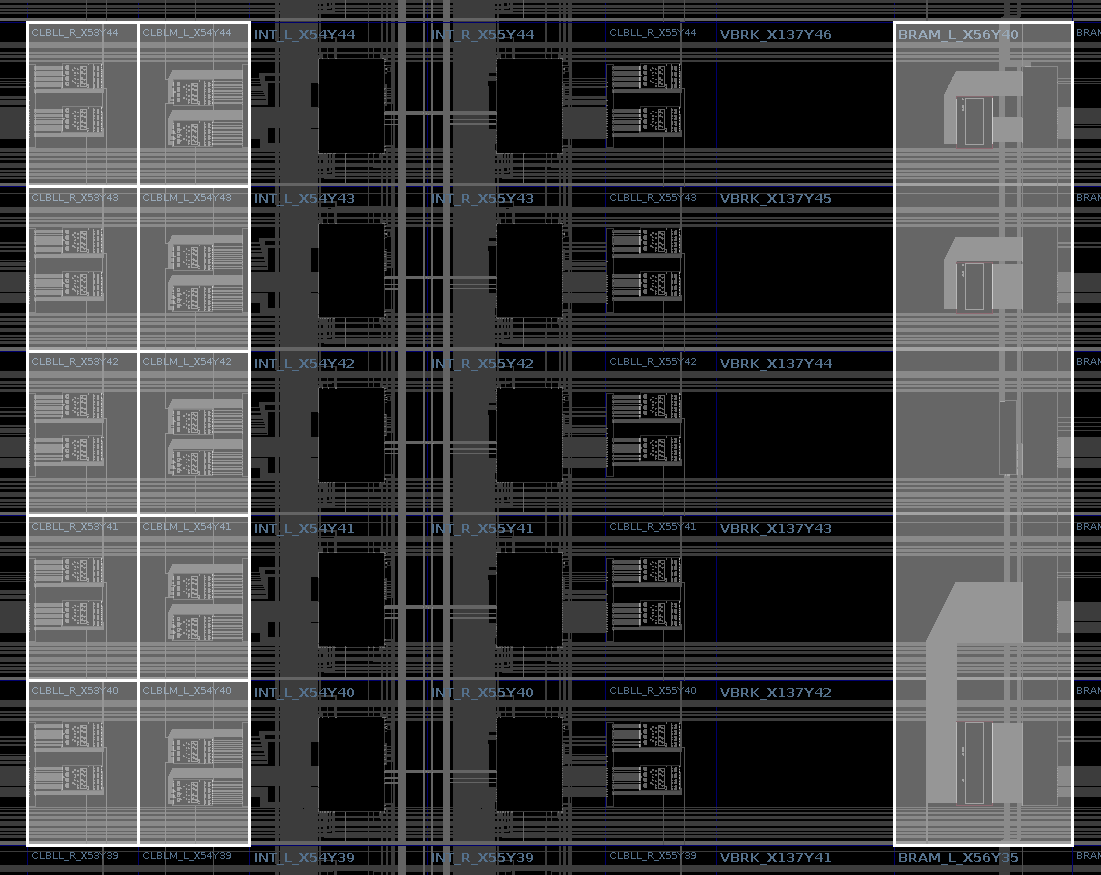
\includegraphics[width=1.25\textwidth]{figures/CLB_BRAM.png}
        \caption{CLB vs BRAM area profile comparison on the xc7z020. 1 BRAM tile highlighted on the right, 10 CLB tiles highlighted on the left.}
        \label{fig:CLB_BRAM}
    \end{figure}

\section{Model Description}
    All Verilog source codes for the implementation can be found in the \texttt{/src/} directory.
    Refer to Figure~\ref{fig:rtl_top_level} for an RTL elaboration schematic for the top\_level module.
    The FIR Filter module on its own communicates via multiple 24-bit data buses.
    Since an FPGA package only has a limited amount of IO pins, we implement serializer-deserializer (SERDES) modules to communicate serially over a simple AXI-like handshake protocol.
    Observe from the top\_level schematic from left to right: input ports which correspond to physical IO pins on the chip, the deserializer, the fir filter itself, the serializer, and finally, the output ports.
    \begin{figure}
        \centering
        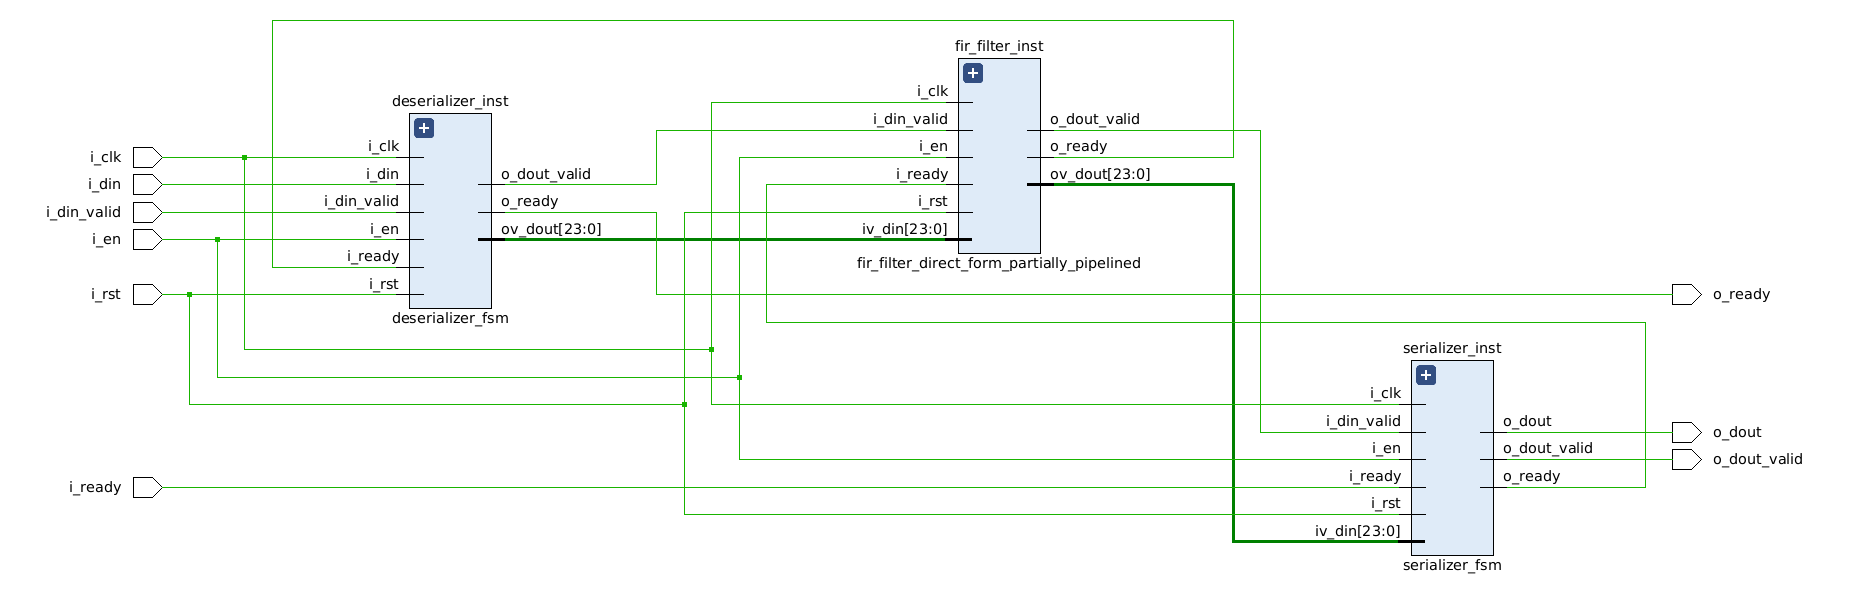
\includegraphics[width=1.4\textwidth]{figures/rtl_top_level.png}
        \caption{top\_level RTL block diagram (auto-generated in Vivado: \texttt{synth -rtl})}
        \label{fig:rtl_top_level}
    \end{figure}

    Shown in Figure~\ref{fig:RAM_ROM_MAC} is a block diagram showing the expandable ROM-RAM-MAC structure for the MAC pipelines.
    In the figure are only the first 3 pipelines, but the pattern for how to expand it to the necessary number of pipelines via should be clear.
    The partial sums on the right-side are summed concurrently in an adder chain.
    Further improvements can be made here in the final summation such as using a binary adder tree.
    \begin{figure}
        \centering
        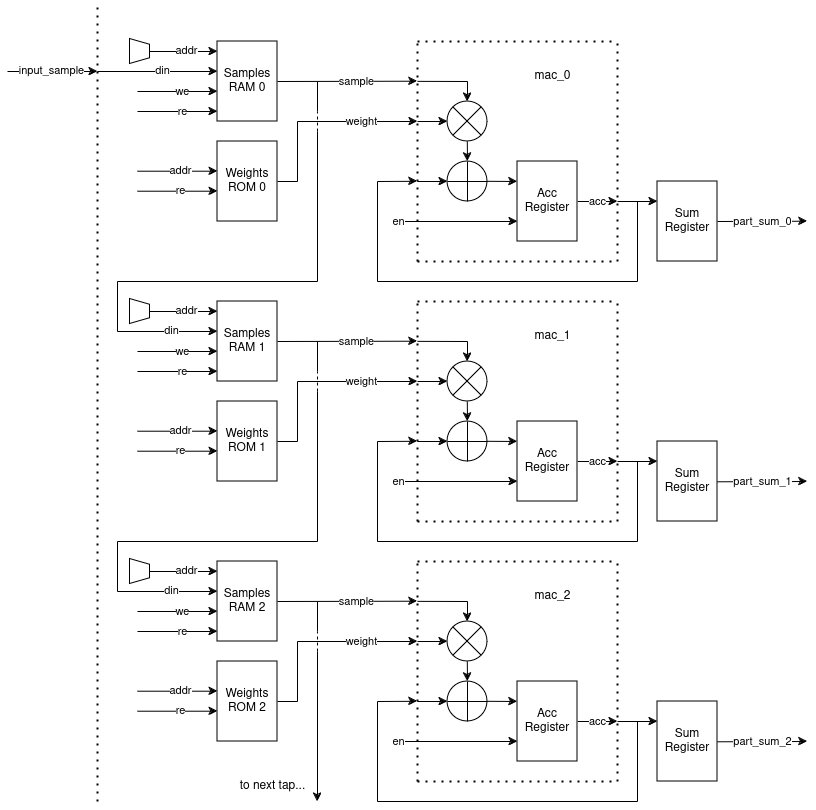
\includegraphics[width=1.25\textwidth]{figures/RAM_ROM_MAC.png}
        \caption{
            Block diagram describing the expandable ROM-RAM-MAC pipeline structure (manually drawn via Draw.io).
        }
        \label{fig:RAM_ROM_MAC}
    \end{figure}

    The full RTL elaborated schematic of the exploded FIR filter module is too large to fit on one screen, but to give an impression,
    shown in Figure~\ref{fig:rtl_fir_closeup} is a closeup of the filter with one pipeline highlited in dark-blue border.
    \begin{figure}
        \centering
        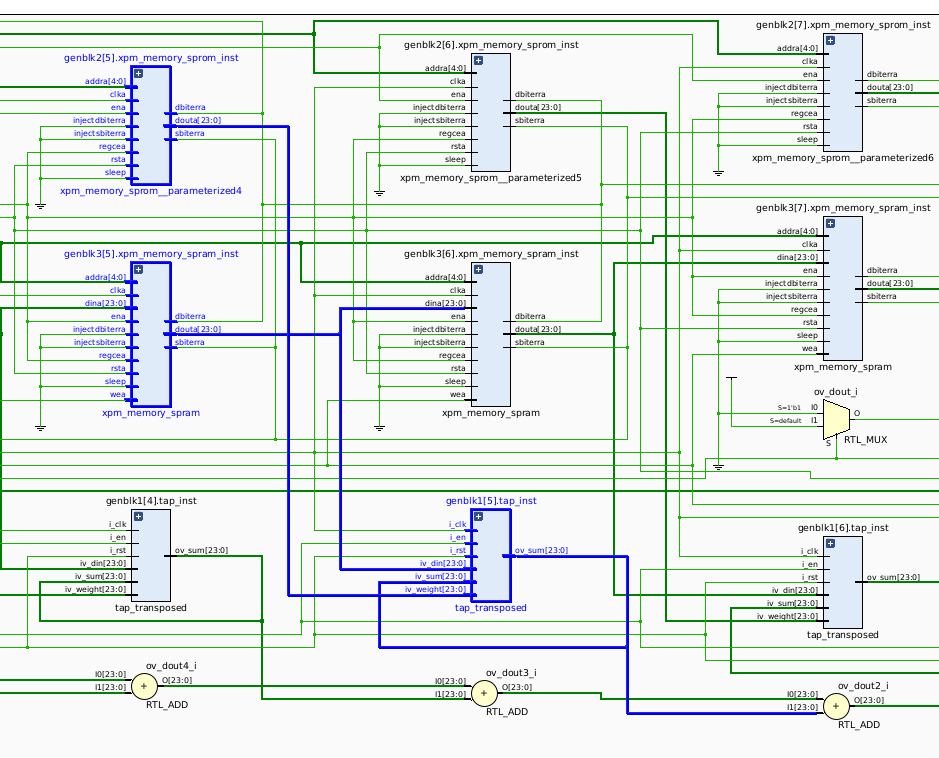
\includegraphics[width=1.25\textwidth]{figures/rtl_fir_closeup.png}
        \caption{
            Closeup of RTL elaboration schematic highlighting one ROM-RAM-MAC pipeline in dark-blue border (auto-generated in Vivado: \texttt{synth -rtl}).
        }
        \label{fig:rtl_fir_closeup}
    \end{figure}

    Shown in Figure~\ref{fig:read_write_operations} is a timing diagram illustrating the write operations for an 8-tap 2-pipeline FIR Filter.
    Every horizontal section divided by dotted lines represents a slice in time corresponding with each write operation.
    Note that t=1,2,.. only corresponds to write operations.
    In between each write operation are \texttt{PIPE\_DEPTH} consecutive read operations, with:

    \[
        \text{PIPE\_DEPTH} = \frac{\text{FIR\_DEPTH}}{\text{PIPELINES}}
    \]

    For simple illustration, the diagram describes an 8-tap filter with just 2 MAC pipelines.
    Thus, PIPE\_DEPTH = 4 in this illustration.
    Each MAC holds 4 input samples and 4 weights.
    The arrows between the RAM and ROM show the corresponding pairs of samples and weights that must be read into the MAC.
    The samples are written into the RAM starting at address = max\_value, in this case, max\_value = 2'b11.

    Then, samples and weights are read consecutively into the MAC with the ROM read address starting at 2'b00 and the RAM read address starting at the write address.
    With each sample, the addresses increment upwards. The RAM read address resets to 2'b00 when it overflows and continues counting upward.
    Then, before the next input sample is received by the filter, the sample to be overwritten in each RAM is written into the RAM of the next pipeline.
    The sample to be overwritten at this point is already on the RAM's data\_out bus and is immediately ready to be written into the next RAM.
    The newly received input sample is then written into the first pipeline RAM.
    Shown in Figure~\ref{fig:read_write_operations} at t=4 illustrates this write-into-next-ram-then-overwrite operation.
    Also note that the RAMs have a separate read address and write address which are multiplexed into its address port.

    This illustration should hopefully suffice in showing how to expand this operation from 8-taps with 2-pipelines to 256-taps with 8-pipelines.

    \begin{figure}
        \centering
        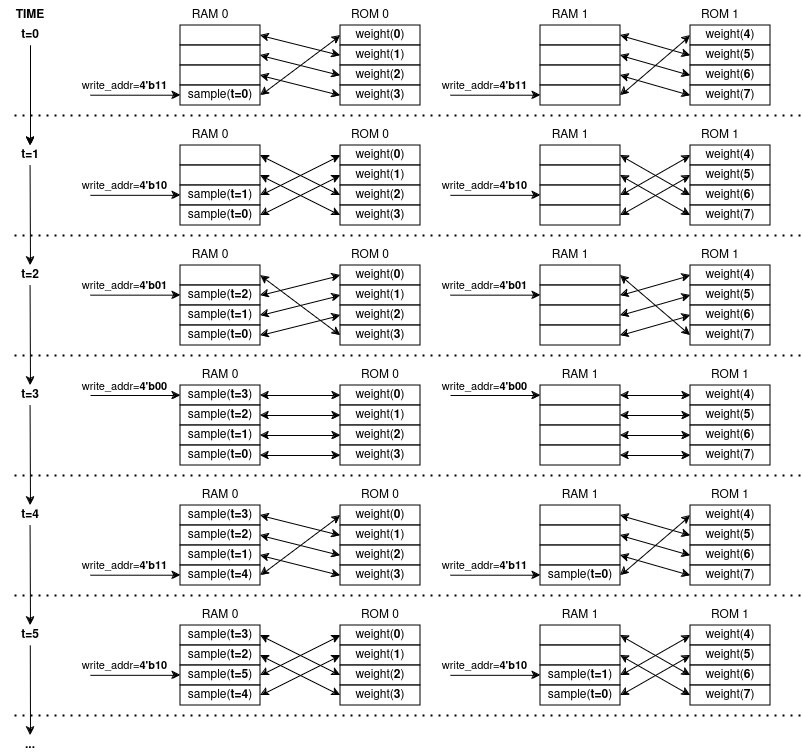
\includegraphics[width=1.25\textwidth]{figures/read_write_operations.png}
        \caption{
            Timing diagram describing the write operation with each incoming input sample for an 8-tap 2-MAC-pipelines FIR Filter (manually drawn via Draw.io).
        }
        \label{fig:read_write_operations}
    \end{figure}


\section{Experimental Procedure and Results}
    As described in the Data Description section,
    we design a testbench that feeds a noisy signal containing a 200Hz sine wave + 5KHz noise sine wave into the design and 
    expect a clean 200Hz sine wave from the output.
    Shown in Figure~\ref{fig:waveform} is the testbench waveform simulation showing the noisy input signal passed into the FIR filter
    and the clean signal output.
    In an industry setting, a more mature verification approach would be to do a spectral analysis on the output signal, likely via Python or Matlab,
    to see what frequency bands have passed the filter.
    Verifying an analog signal via waveform diagrams is just a quick-and-dirty way to demonstrate the basic principles of the low-pass filter.

    \begin{figure}
        \centering
        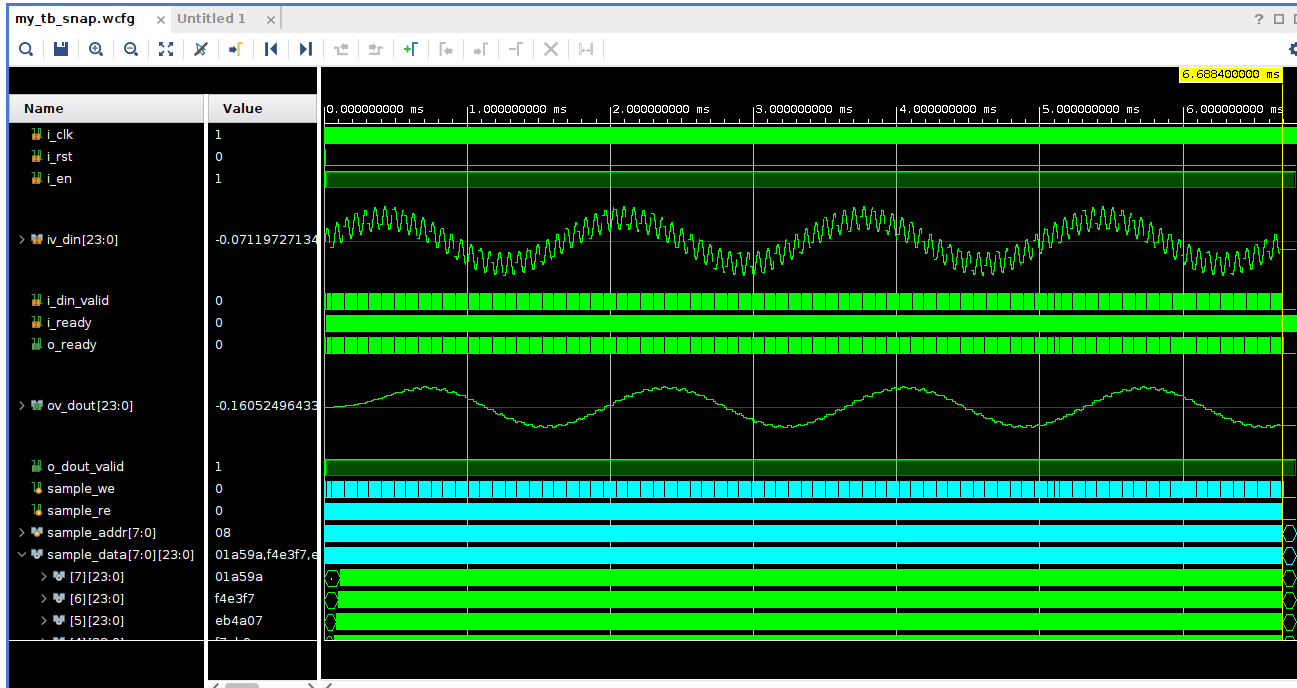
\includegraphics[width=1.25\textwidth]{figures/waveform.png}
        \caption{
            Testbench waveform simulation showing the noisy input signal iv\_din and clean output signal ov\_dout.
        }
        \label{fig:waveform}
    \end{figure}

    Shown in Figure~\ref{fig:utilization} is the resource utilization report summarizing the number of LUTs, FFs, DSPs, and BRAMs used.
    Note that BMEM count shows 8, but after inspecting the netlist, I can confirm that 16 BRAM BELs are indeed used.
    I am not entirely sure what BMEM is or how it is counted.
    \begin{figure}
        \centering
        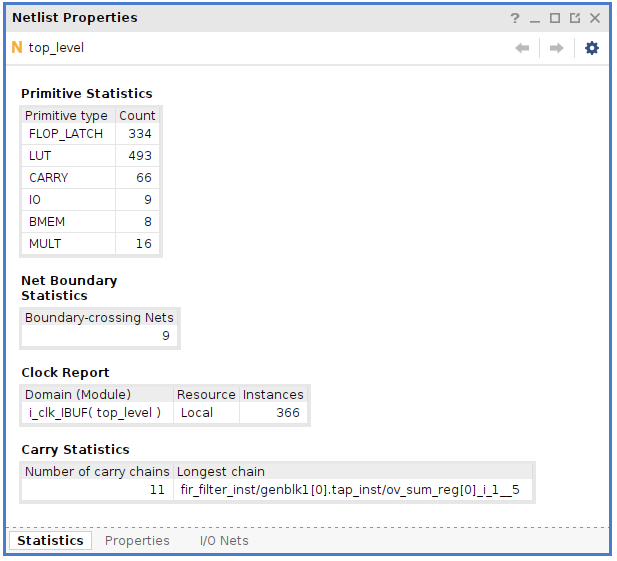
\includegraphics[width=0.75\textwidth]{figures/utilization.png}
        \caption{
            Synthesis resource utilization report.
        }
        \label{fig:utilization}
    \end{figure}

    Shown in Figure~\ref{fig:device} is the design placed and routed onto the xc7z020 using the default Vivado implementation strategy.
    \begin{figure}
        \centering
        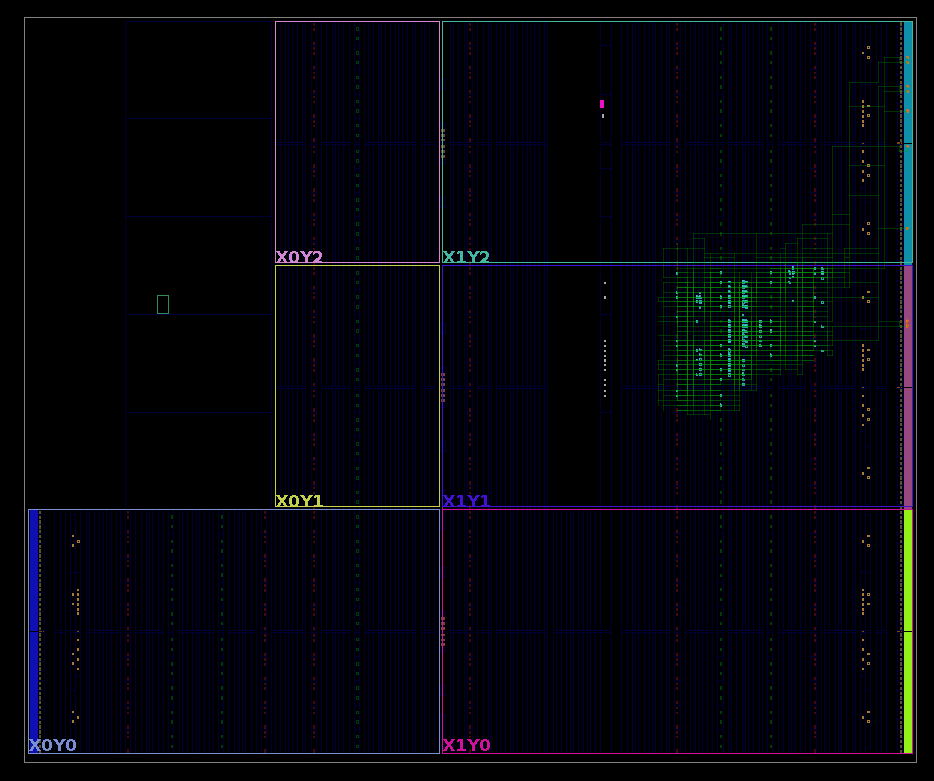
\includegraphics[width=1.25\textwidth]{figures/device.png}
        \caption{
            The final design placed and routed onto the xc7z020 via Vivado default implementation strategy.
        }
        \label{fig:device}
    \end{figure}
    Shown in Figure~\ref{fig:timing} is the timing report with the clock constraint set to 10MHz.
    With a worst negative slack of +87ns which represents the critical path delay of the design,
    we can likely increase our clock speed without penalty if higher performance is needed.
    \begin{figure}
        \centering
        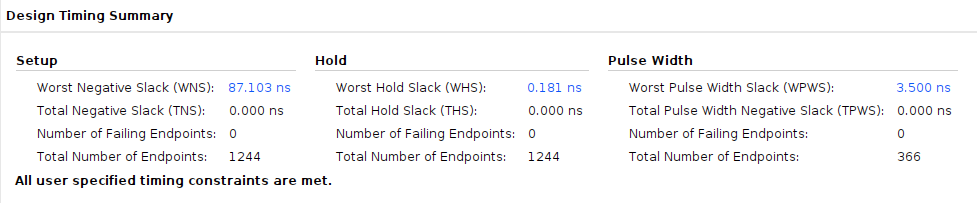
\includegraphics[width=1.25\textwidth]{figures/timing.png}
        \caption{
            Timing report shoing critical path delay (Worst Negative Slack)
        }
        \label{fig:timing}
    \end{figure}

    I have not used the Power report summary in Vivado before and not familiar with the report methodology, 
    so I cannot offer concrete commentary on the power usage.
    However, to give some impression, shown in Figure~\ref{fig:power_breakdown} and Figure~\ref{fig:power_environment} 
    are the power breakdown and environment settings.
    At a glance, it seems that BRAM usage takes up a lionshare of 44\% of the power usage.
    Using 16 BRAM sites in our partially pipelined implementation replaced 6144 flip-flops of a 
    traditional direct-form implementation as discussed in the Method Description section.
    From the utilization report, 334 FLOP\_LATCH (Flip Flops) were used.
    From the power report breakdown, I assume flip flop power usage is represented by Clocks and Signals which use 5\% and 16\% respectively, 
    summing up to 21\%.
    Had we used the traditional direct-form implementation and added 6144 additional flip-flops to the design, 
    I suspect they may have used a larger percentage of the power.
    \begin{figure}
        \centering
        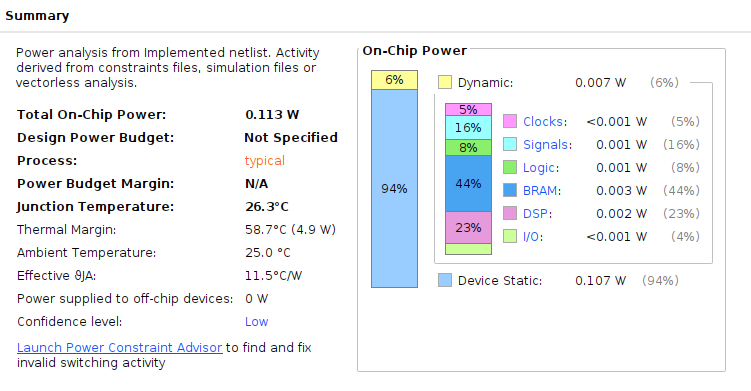
\includegraphics[width=1.00\textwidth]{figures/power_breakdown.png}
        \caption{
        }
        \label{fig:power_breakdown}
    \end{figure}
    \begin{figure}
        \centering
        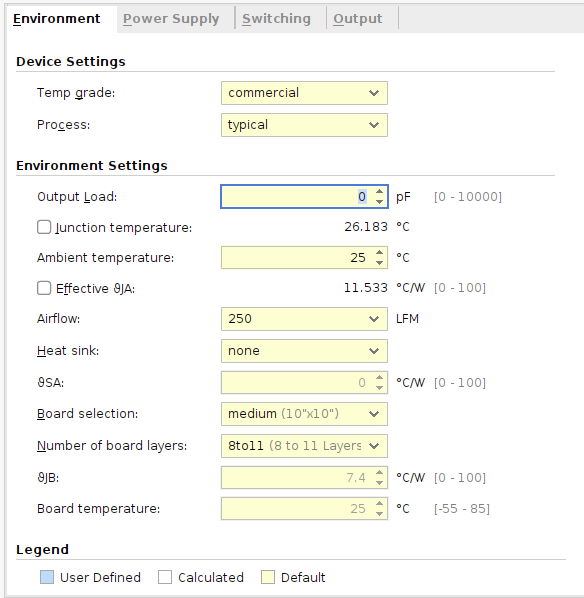
\includegraphics[width=0.60\textwidth]{figures/power_environment.png}
        \caption{
        }
        \label{fig:power_environment}
    \end{figure}


\section{Conclusion}
    This paper presented a RAM-based partially pipelined Verilog model of an FIR Filter whose data width, filter depth, and number of pipelines
    can be easily reconfigured via the top\_level parameters.
    We have also demonstrated a 24-bit 256th order low-pass filter with 8 parallel MAC pipelines and performed a simple testbench simulation to verify its functionality.
    There is certainly many improvements that could be done with this Verilog model in the future.

    As mentioned before, the final summation of the partial sums from each MAC pipeline are summed in one clock cycle via adder chain.
    One could improve upon this by using a binary adder tree and introducing some pipelining along the tree stages.
    However, the FPGA CARRY4 BELs in modern 7-series FPGAs are very optimized, and the fact that our throughput is likely
    limited by BRAM memory access suggests that this is probably not the bottleneck.
    I suspect the limiting factor in terms of throughput is indeed the BRAM memory access.
    If BRAM access becomes a problem, then the designer will have to increase the number of MAC pipelines to exploit the parallel time-slice processing.

    Another consideration would be to explore the usage of Distributed RAMs mentioned previously to forego expensive BRAMs entirely.
    The SLICEM logic sites have special LUTs that can be reconfigured as small local LUTRAMs.
    Some more implementations can be set up to see if this could keep CLB usage low while avoiding BRAM.

    As mentioned in the Experiments and Results section, a more mature verification environment can be employed to really stress-test the filter
    and to run batches of tests with various random input signals to really see the band of frequencies that passes through the filter.
    This could also help us in verifying the frequency response and to judge the signal to noise ratio of the signal.

    A more in-depth exploration of the power usage and the QoR of the placement and routing is also due.


\newpage
\section{References}
    \bibliographystyle{ieeetr}
    \nocite{*}
    \bibliography{
        references/references
    }


\end{document}
